\section{Results}
\label{sec:results}

\subsection{Diffusion equation}

In Figure \ref{fig:FDcompare} two different instants in the time evolution of the diffusion equation (eq. \ref{eq:diffusionEQ}), as obtained from finite difference methods, are shown. For both, a comparison is made with the exact solution and a run with higher spatial resolution. In both cases, the graphs are difficult to distinguish, except for the lower resolution run, which is not as smooth.
 \begin{figure}[htbp]
  	\centering
  	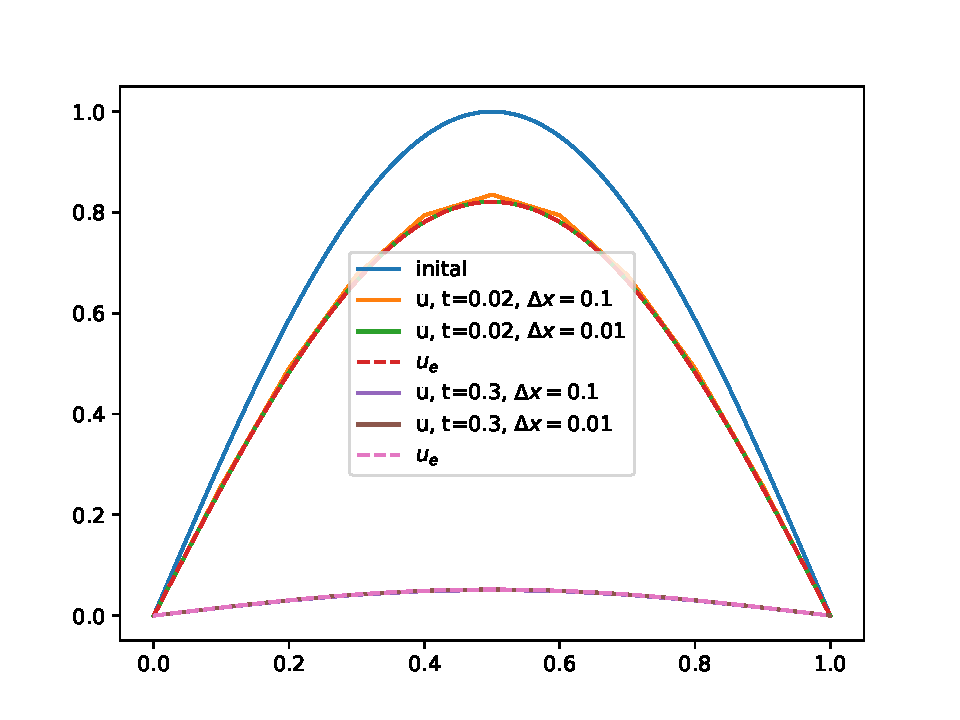
\includegraphics[width=0.5\textwidth]{FD_solved}
  	\caption{Time evolution of eq. \ref{eq:diffusionEQ} solved using finite difference methods: CD and FE. For each point in time a visual comparison is made with the exact solution, represented by dashed lines, as well as a run with higher spatial resolution, represented by different colours.}
   \label{fig:FDcompare}
 \end{figure}

Likewise, in Figure \ref{fig:NNcompare} we show a parallell to Figure \ref{fig:FDcompare} with solutions from a neural network. In this case, we also see agreement between the computed and exact solutions for both points in time.
 \begin{figure}[htbp]
  	\centering
  	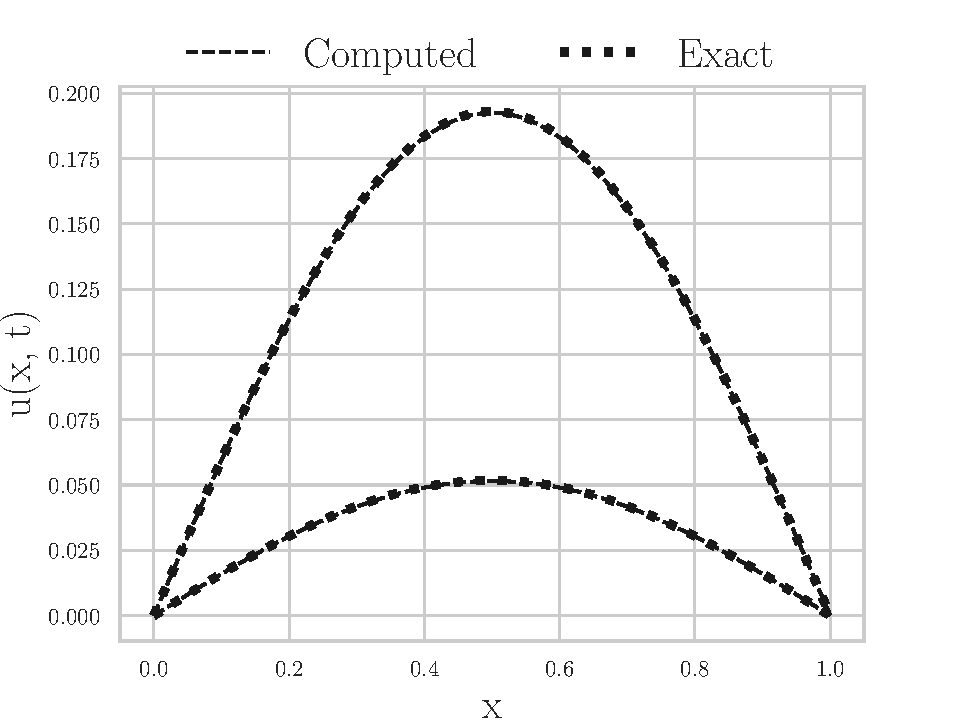
\includegraphics[width=0.5\textwidth]{NN_solved}
  	\caption{Time evolution of eq. \ref{eq:diffusionEQ} solved using a neural network. For both instants in time, a visual comparison is made with the exact solution, represented by dashed lines.}
   \label{fig:NNcompare}
 \end{figure}

Shown in Figure \ref{fig:MSEbench} are the MSE's for two instants in time for both finite difference methods and a neural network. For the finite difference methods we observe a decrease in MSE for increasing temporal solution, slowing down after around 500 time points for both cases. For $t=0.02$ s (a.), the MSE is minimal at around $10^{-6}$ for 1000 time points, while for $t=0.3$ s (c.) it only becomes around $10^{-5}$ for 1000 time points.

For the neural network, we observe a decrease in MSE for an increasing number of iterations. In the case of $t=0.02$ s (b.), we see that the MSE decreases below $10^{-8}$ after around 6000 iterations, with a further, but slight, decrease at 10000 iterations. As for $t=0.3$ s (d.), the MSE is below $10^{-8}$ after around 4000 iterations and is mostly unchanged afterwards.

Comparison between the finite difference methods and the neural network, we see that the neural network can obtain an MSE 2-3 orders of magnitude lower than the finite difference methods.
\begin{figure}[htbp]
 	\centering
 	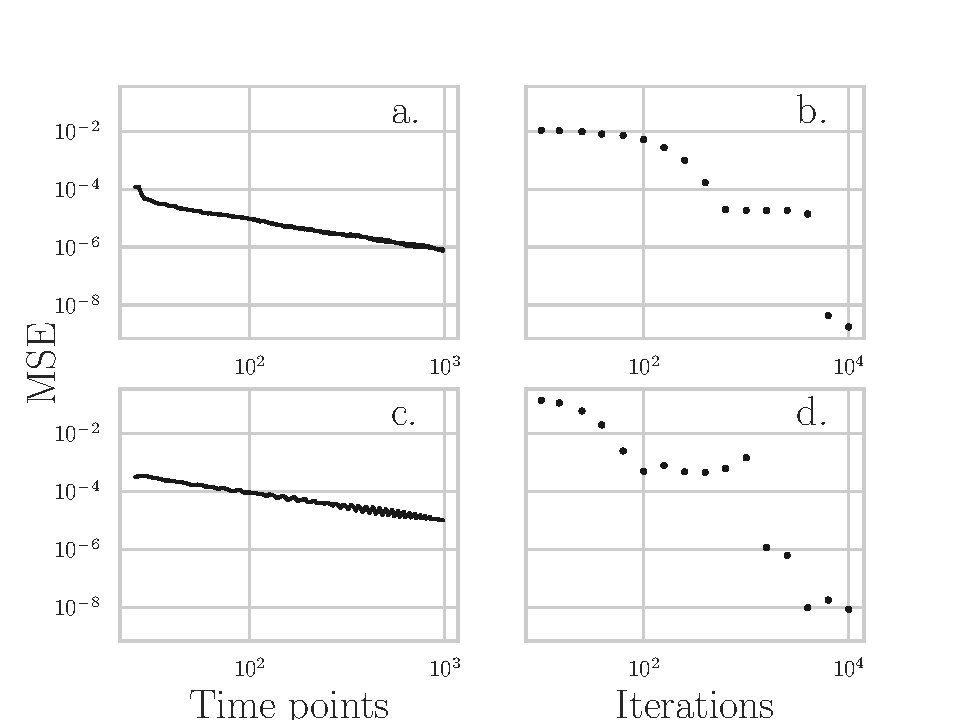
\includegraphics[width=0.5\textwidth]{MSEbench}
  \caption{Shown on the left-hand side, top-to-bottom (a., c.), are the MSE's as a function of temporal resolution, obtained from using finite difference methods for $t=0.02$ and $t=0.3$, respectively. Likewise, on the right-hand side (b., d.) the MSE's yielded from the neural network are shown as a function of iterations with network parameters $N_t = 10$, $N_x = 100$, and $\gamma = 0.004$.}
  \label{fig:MSEbench}
\end{figure}

Accompanying Figure \ref{fig:MSEbench}, we show the CPU times as a function of temporal resolution and number of iterations, respectively, for the different scenarios in Figure \ref{fig:CPUbench}. We see that the general curve is very similar for all scenarios. For the CD/FE method, we see that the CPU time becomes slightly longer for shorter t at 1000 time points. The neural network looks to have the same curve in both b. and d.

Comparing the two methods, we see that the neural network is around 3 orders of magnitude, if not more, slower than the finite difference methods.
\begin{figure}[htbp]
 	\centering
 	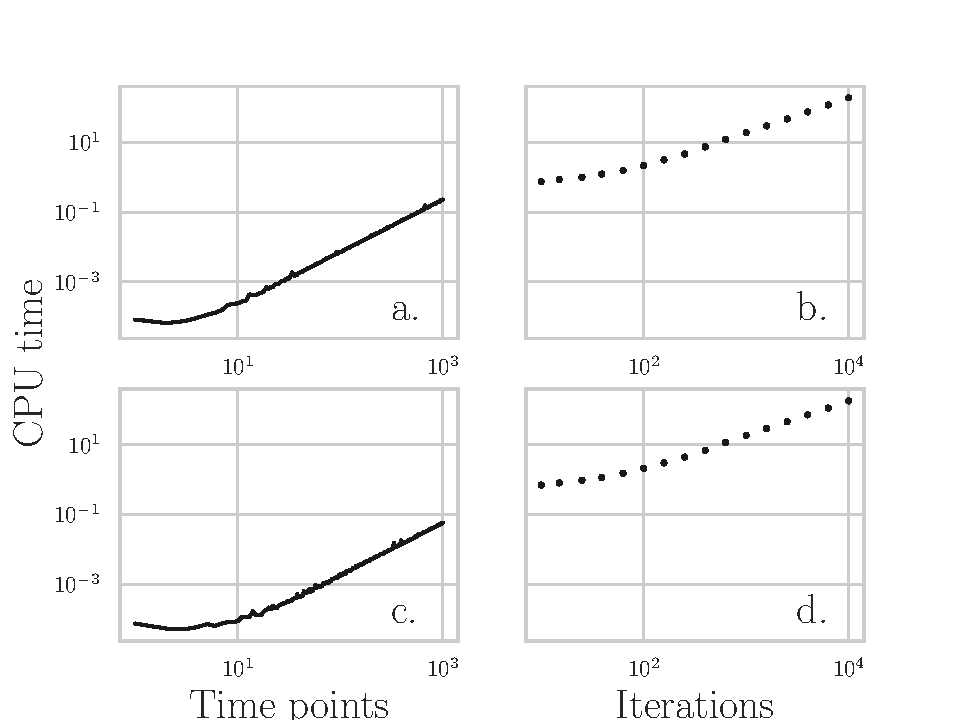
\includegraphics[width=0.5\textwidth]{CPUbench}
 	\caption{Shown on the left-hand side, top-to-bottom (a., c.), are the CPU time's as a function of temporal resolution, obtained from using finite difference methods for $t=0.02$ and $t=0.3$, respectively. Likewise, on the right-hand side (b., d.) the CPU time's yielded from the neural network are shown as a function of iterations with network parameters $N_t = 10$, $N_x = 100$, and $\gamma = 0.004$.}
  \label{fig:CPUbench}
\end{figure}


\subsection{Eigenpairs}

\begin{equation*}
v_{max}^{np} = \begin{bmatrix}
	0.4025950 \\
	0.4790814 \\
	0.3357358 \\
    0.3835011 \\
    0.3542414 \\
    0.4723555
\end{bmatrix} \quad w_{max}^{np} =  2.83515
\end{equation*}

\begin{equation*}
v_{max}^{nn} = \begin{bmatrix}
	0.4023249 \\
	0.4791663 \\
	0.3364637 \\
	0.3822769 \\
	0.3541386 \\
	0.4730503
\end{bmatrix} \quad w_{max}^{nn} = 2.83514
\end{equation*}\begin{equation*}
v_{max}^{np} = \begin{bmatrix}
	0.4025950 \\
	0.4790814 \\
	0.3357358 \\
    0.3835011 \\
    0.3542414 \\
    0.4723555
\end{bmatrix} \quad w_{max}^{np} =  2.83515
\end{equation*}

\begin{equation*}
v_{max}^{nn} = \begin{bmatrix}
	0.4023249 \\
	0.4791663 \\
	0.3364637 \\
	0.3822769 \\
	0.3541386 \\
	0.4730503
\end{bmatrix} \quad w_{max}^{nn} = 2.83514
\end{equation*}

\begin{figure}[htbp]
 \centering
 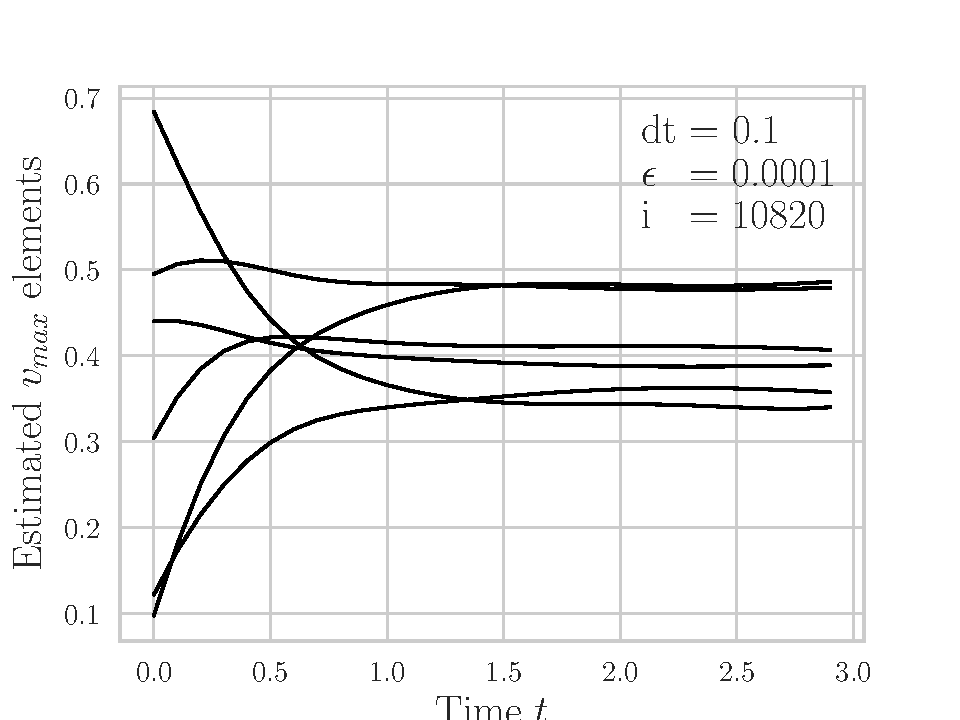
\includegraphics[width=0.5\textwidth]{eigenvector_max}
 \caption{Figure showing how the value of the elements of the estimated eigenvector $v_{max}$ evolves over time. Each line represents one of the elements of the vector.}
 \label{fig:eigenvector_max}
\end{figure}


\begin{equation*}
  v_{min}^{np} = \begin{bmatrix}
   0.6928048 \\
  -0.0074343 \\
  -0.7048516 \\
  -0.1487365 \\
  0.0122096 \\
  0.0296413
  \end{bmatrix} \quad w_{min}^{np} = -0.515594
\end{equation*}

\begin{equation*}
  v_{min}^{nn} = \begin{bmatrix}
   -0.69116113  \\
   0.00492352  \\
   0.70646873  \\
   0.14887754 \\
   -0.01982836 \\
   -0.02482513
  \end{bmatrix} \quad w_{min}^{nn} = -0.515528
\end{equation*}

\begin{figure}[htbp]
 \centering
 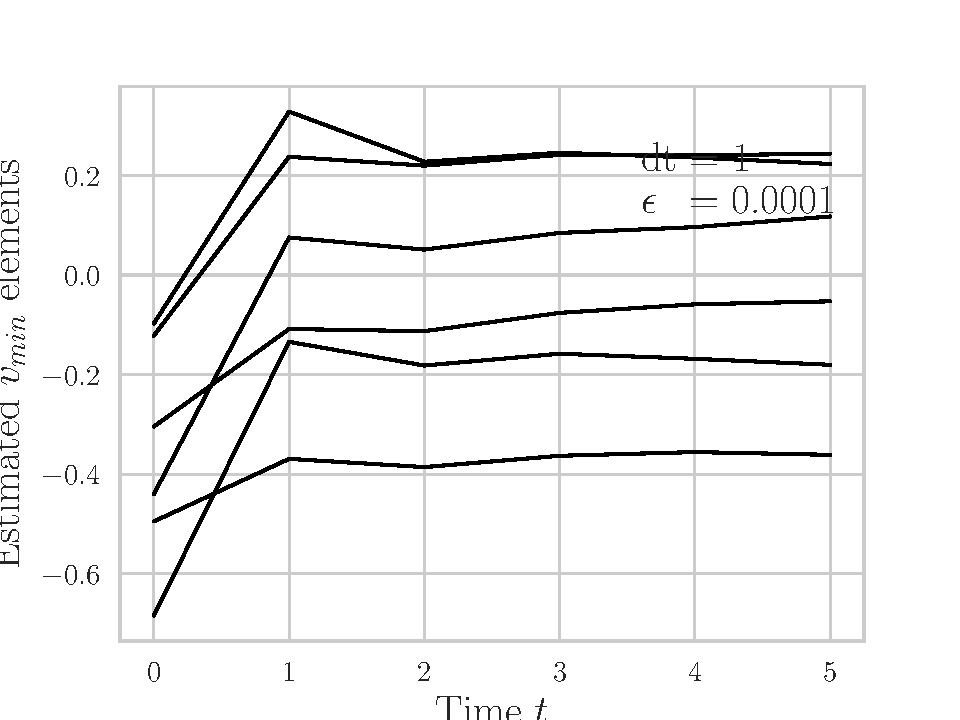
\includegraphics[width=0.5\textwidth]{eigenvector_min}
 \caption{Figure showing how the value of the elements of the estimated eigenvector $v_{min}$ evolves over time. Each line represents one of the elements of the vector.}
 \label{fig:eigenvector_min}
\end{figure}

% Eksempel for figurer
% \begin{figure}[htbp]
% 	\centering
% 	\includegraphics[width=0.5\textwidth]{}
% 	\caption{}
% 	\label{fig:}
% \end{figure}
